\section{The SOM learning algorithm}

\mode<presentation>{
\begin{frame} 
    \begin{center} \huge
        \secname
    \end{center}
    \begin{center}
		Compete, Cooperate and Adapt\\
		Learn to ``cover''/``explain'' the data
    \end{center}
\end{frame}
}

% --------------------------------------------------------------------------
\begin{frame}[shrink=1] 
\begin{figure}[!th]
\footnotesize
\removelatexerror
\begin{algorithm}[H]
\DontPrintSemicolon  
\textbf{Initialization:} \;
- choose no. $M$ of partitions (``neurons'') \textcolor{red}{and the topology of the map}\;
- choose annealing schedule for $\varepsilon$ and $\sigma$\;
- initialize $M$ prototypes: $\vec{w}_{\vec q} = 1/p \sum_\alpha \vec{x}^{(\alpha)}+\vec{\eta} $, \hspace{0.3cm}$\vec{\eta}$ small noise vector \;
\Begin(){
  choose a random data point $\vec{x}^{(\alpha)}$ \\
  determine the closest prototype:\[ \vec{p} = \underset{\vec r}{\argmin} \big| \vec{x}^{(\alpha)} - \vec{w}_{\vec r} \big|\] \\
  change all prototypes $\vec{w}_{\vec q}$ according to: $$\Delta \vec{w}_{\vec q} = \varepsilon \cdot h_{\vec{q} \, \vec{p}} \cdot 
  \big( \vec{x}^{(\alpha)} - \vec{w}_{\vec q} \big) \text{\hspace{1cm} for \textcolor{red}{all} \vec{q}}$$ \\
  lower the learning rate $\varepsilon$ and neighborhood width $\sigma$
}
\label{alg:kohonen}
\caption{On-line learning for SOM}
\end{algorithm}
\end{figure}

\end{frame}

\subsection{The neighborhood function}

% --------------------------------------------------------------------------
\begin{frame}[t] \frametitle{\subsecname~$h_{\vec{q} \, \vec{p}}$} 
\begin{equation}
	\Delta \vec{w}_{\vec q} = \varepsilon \cdot h_{\vec{q} \, \vec{p}} \cdot
  \big( \vec{x}^{(\alpha)} - \vec{w}_{\vec q} \big) \text{\hspace{1cm} for \textcolor{red}{all} q}
  \end{equation}
\begin{itemize}
	\item $h_{\vec{q} \, \vec{p}}$ enforces similar learning steps for neighboring neurons
	\item common choice:
	\begin{equation}
		h_{\vec{q} \, \vec{p}} = \exp \bigg\{ - \frac{ (\vec{q}
			- \vec{p} )^2 }{2 \sigma^2} \bigg\}
			\end{equation}
\end{itemize}

\begin{center}
\begin{minipage}{0.4\textwidth}
\begin{center}
	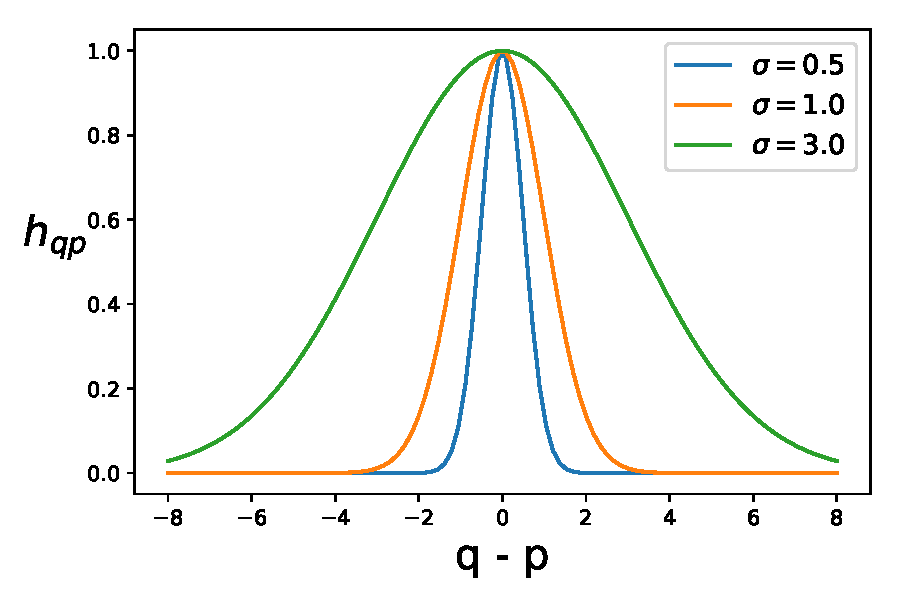
\includegraphics[width=0.9\textwidth]{img/guassian_function_1d}
	\notesonly{\captionof{figure}{In the case of a 1D map}}
\end{center}
\end{minipage}
\begin{minipage}{0.4\textwidth}
\begin{center}
	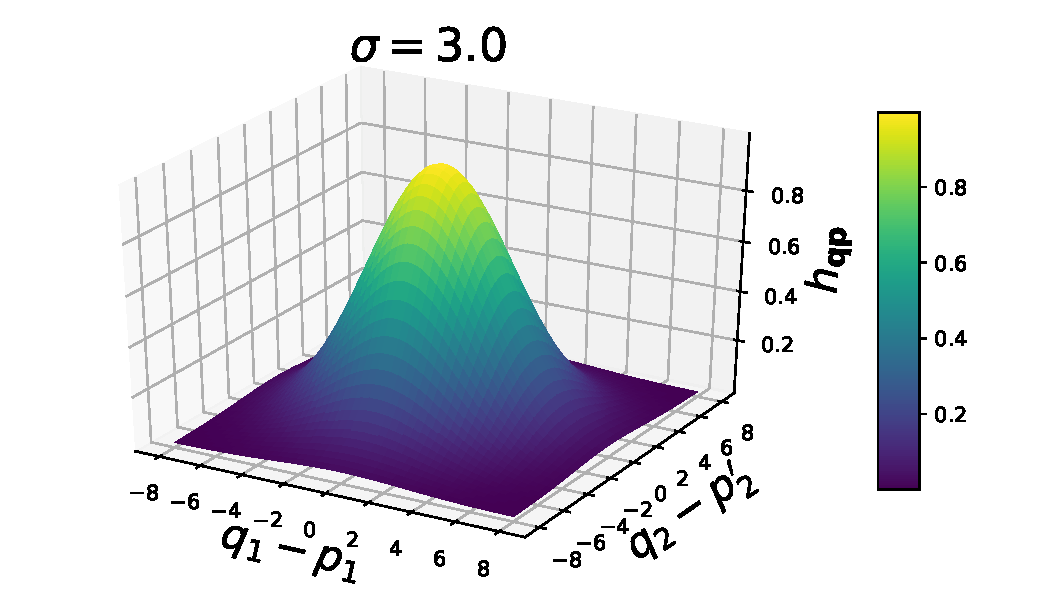
\includegraphics[width=0.9\textwidth]{img/guassian_function_2d_3Dview}
	\notesonly{\captionof{figure}{In the case of a 2D map}}
\end{center}
\end{minipage}
	\notesonly{\captionof{figure}{The Gaussian function around the winning neuron.}}
\end{center}

\end{frame}

\begin{frame}[t] \frametitle{\subsecname~$h_{\vec{q} \, \vec{p}}$} 

\svspace{-5mm}

\begin{center}
	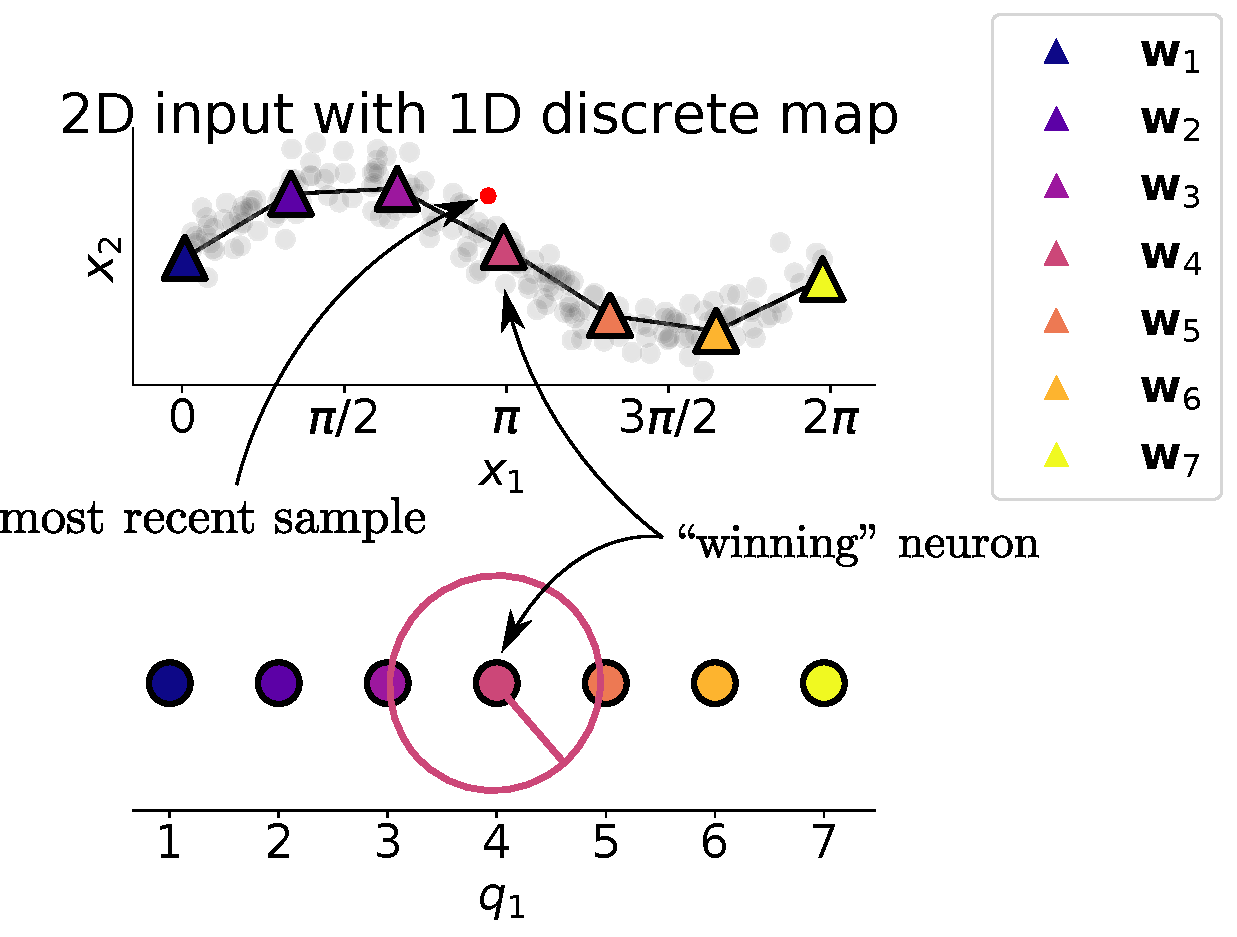
\includegraphics[width=0.44\textwidth]{img/sin_manifold_map_rbf}
	\notesonly{\captionof{figure}{The role of the neighborhood function}}
\end{center}


\svspace{-3mm}


\slidesonly{
\begin{equation}
	\Delta \vec{w}_{\vec q} = \varepsilon \cdot h_{\vec{q} \, \vec{p}} \cdot
  \big( \vec{x}^{(\alpha)} - \vec{w}_{\vec q} \big) \text{\hspace{1cm} for \textcolor{red}{all} q}
  \end{equation}
}

\svspace{-3mm}

\question{What is the effect of the width $\sigma$?}

\begin{itemize}
    \item<only@2,3> large $\sigma$ (very wide width): \only<3>{all neurons will move towards the new point.}
    \item<only@4,5> $\sigma \rightarrow 0$: \only<5>{standard on-line K-means (only update $\vec{q}=\vec{p}$)}
\end{itemize}

\end{frame}


% --------------------------------------------------------------------------
% --------------------------------------------------------------------------
\begin{frame}[t] \frametitle{\subsecname~$h_{\vec{q} \, \vec{p}}$} 
\slidesonly{
$$		h_{\vec{q} \, \vec{p}} = \exp \bigg\{ - \frac{ (\vec{q}
			- \vec{p} )^2 }{2 \sigma^2} \bigg\}
$$
}
\emph{$\sigma$ annealing}
\begin{itemize}
      \itr start with large
        $\sigma$  ($\leadsto$ neighborhood function convex over
        its support)
      \itr decrease linearly or exponentially (but
        ``slowly'') during learning.
       \itr solution depends on 
        final value of $\sigma$
        \vspace{0.5cm}
       \itr $\sigma \rightarrow 0$: minimum of the K-means clustering cost function but 
            \emph{``neighborhood preserving''}  \itr $\sigma$ small : better representation capabilities at the expense of a non-optimal clustering cost 
\end{itemize}

\question{What happens when we rush the annealing process?}

\end{frame}

\begin{frame}{The effect of rushing the annealing process}


- We ``leave the neighborhood behind''. It ``kicks into K-means mode'' too early.

\begin{minipage}{0.45\textwidth}
\begin{center}
	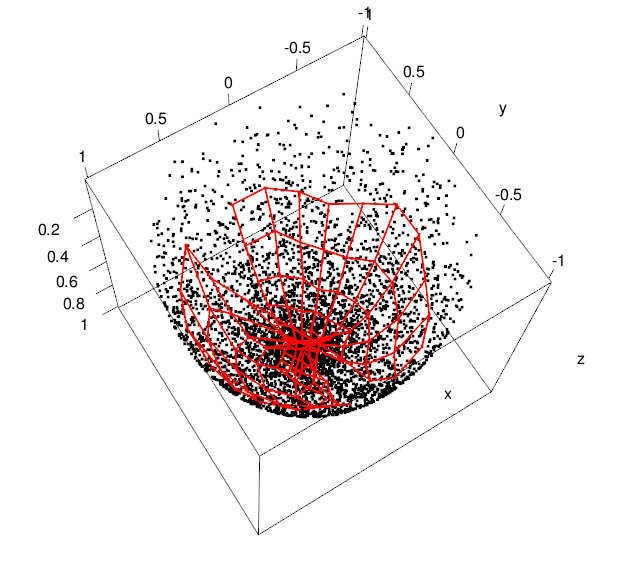
\includegraphics[width=0.9\textwidth]{img/3-bowlS2-2}
	\notesonly{\captionof{figure}{Slow annealing process preserves the neighborhood among the neurons}}
\end{center}
\end{minipage}
\begin{minipage}{0.45\textwidth}
\begin{center}
	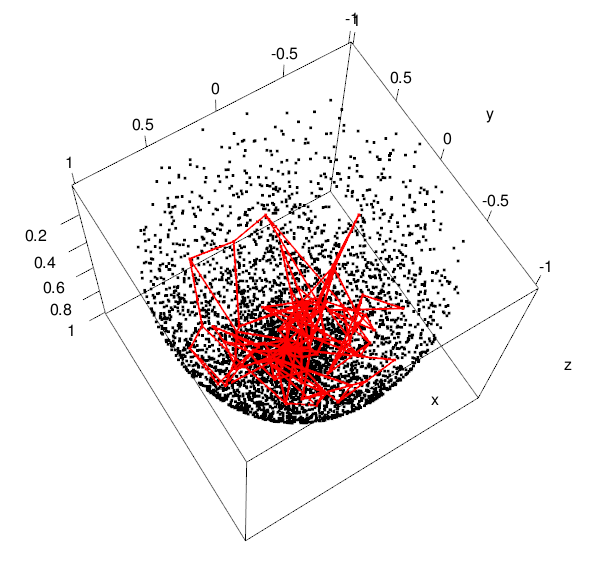
\includegraphics[width=0.9\textwidth]{img/3-bowlS2-1}
	\notesonly{\captionof{figure}{Annealing too fast ``leaves the neighborhood behind''}}
\end{center}
\end{minipage}

\end{frame}

